\clearpage
\section{Hintergrundstrahlung}

In diesem Versuchsteil geht es darum die Hintergrundstrahlung zu ermitteln, welche in der Messapparatur vorhanden ist. Dazu haben wir 
den Detektor ohne Quelle, aber mit Verschluss positioniert und über Nacht gemessen. Die Messzeit betrug 72000s (totzeitkorrigiert), um auch erst 
spät erkennbare Peaks aufzulösen. 

Die Messung ergab folgendes Bild: Abb. \ref{bild:untergrund}.

\begin{figure}[ht]
    \captionsetup{justification=centering,margin=2cm}
    \centering
    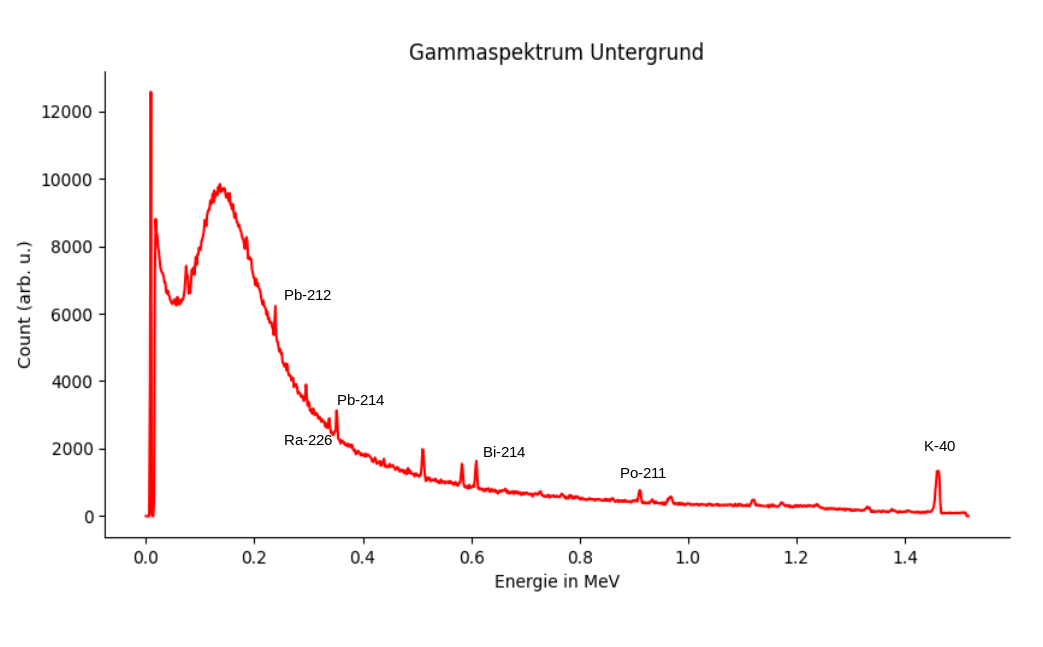
\includegraphics[angle = 90, width = 12cm]{Bilder/Auswertung/Untergrund.png}
    \caption{Untergrundspektrum mit Zuordnung der dazugehörigen Isotope \protect \footnotemark. Manche Linie – beispielsweise 
    die Linien zwischen der Pb-214 und der Bi-214 Linie sind nicht zuordnenbar}
    \label{bild:untergrund}
\end{figure}
\footnotetext{\url{https://hps.org/publicinformation/ate/q7546.html}}
Dabei wurde die obige Internetquelle und eine Literaturquelle (\cite{Mende2016}) verwendet.
Wir hätten im Spektrum der Hintergrundstrahlung Pb-212, Pb-124, Bi-214, K-40 und Ra-220 identifiziert.